\section{Proposed Method}
\label{sec:method}

\subsection{Preliminaries: The Traditional CL Objective}
Let $t=1,2,\ldots$ index the tasks, with $\T(t) = \{\tsk(1), \ldots, \tsk(t)\}$ denoting the task set observed up to time $t$. In a specific experimental setup, tasks arrive according to a permutation $\perm$, where $\perm[i]$ is the index of the task at step $i$ and $\D_{\perm[i]}$ is its dataset. A CL learner is a parametric model with weights $\w \in \R^\pdim$ that must learn each new task $\tau(t)$ without forgetting prior tasks in the sequence.

{The classical goal of a CL learner} is to train a single set of parameters $\w$ given $\perm$ using a cumulative loss~(also called forgetting loss in CL) $\J$ to achieve the following objective 
\begin{align}
    \label{eq:standCL}
   min_{\w} \left\{ \J_{\perm}{(\w)} := \sum_{i=1}^{t} \loss(\w, \D_{\perm[i]}) \right\},
\end{align}
where $\loss$ is the loss function for a specific task. After repeated updates, the learner seeks to attain $\wopt$ that minimizes $\J_{\perm}(\w)$. If the task order is shuffled, with $\pi(t)^{(1)} \ne \pi(t)^{(2)}$, the learner may yield a completely different solution %
to \eqref{eq:standCL} with distinct $J_{\pi(t)^{(1)}}$ and $J_{\pi(t)^{(2)}}$. Empirical evidence demonstrates large variance for two distinct permutations $\perm^{(1)}$ and $\perm^{(2)}$(see Appendix~\ref{app: task-order-impact}).

\subsection{HTCL Formulation: A New Objective}
\label{sec:problem_formulation}
Let $\permset = \{\perm^{(1)}, \ldots, \perm^{(t!)}\}$ denote the set of all $t!$ permutations of the $t$ observed tasks, where each $\perm^{(i)}$ is a complete ordering in which every task appears exactly once. To address the curse of task ordering, it is desirable that $\wopt$ is order/permutation invariant where we minimize \textbf{expected value} of the loss over $\permset$ such that
\begin{align}
    \label{eq:tiCL}%
    \J^{*}(\wopt) = \min_{\w} \, \E_{\perm \sim \permset}\!\left[\J_{\perm}(\w)\right].
\end{align}

\textbf{Intractable combinatorial challenge:}  However, this goal leads to a combinatorial search space. For instance, if $t=20$ tasks, the size of $\permset$ becomes $20! \approx 2.4 \times 10^{18}$. Moreover, as evaluating each sequence requires full training with complete datasets for all the tasks at once, the compute and memory requirements are significant.

\textbf{Tractable optimization problem with a divide and conquer strategy.} To avoid evaluating the full factorial space, which entails over $3.6$ million permutations for $t=10$, we collect $\gsize$ tasks online and perform training. Let the group of $\gsize$ tasks be indicated by $\G.$ Then, for a sequence of $10$ tasks, collecting only two tasks at a time reduces the complexity from $10!$  to just $5 \times 2! = 10.$  In particular, from $\mathcal{O}(\ntasks!)$ to $\mathcal{O}(\ngroups \cdot \gsize!),$ where $\ngroups$ refers to the number of groups formed online as the tasks arrive. 

Moreover, training on the best-performing order within each group eliminates intra-group ordering variance, since the per-group selection rule returns the same model irrespective of the arrival order of tasks within the group. Figure~\ref{fig:new-cl-goal} gives us an overview of how shifting to this new formulation reduces the variance. The theoretical lower bound for the performance improvement due to the group size are established in Theorem~\ref{prop:group_vs_random} (see Appendix~\ref{app:performance-bounds}). In particular, Theorem~\ref{prop:group_vs_random} guarantees that HTCL's per-group selection meets or exceeds the expected accuracy under a uniformly random choice of intra-group orderings. %

However, when the next group of tasks are available this order invariance must be retained while training on the next group. Towards this end, we introduce a hierarchical strategy that aggregates the information from new group without losing order invariance from the previous group. 

\subsection{The HTCL Framework: Decoupling Plasticity and Stability}
\label{sec:htcl_framework}

Once the first group of tasks was observed, we solved \eqref{eq:tiCL}  and obtained $\wl^{1}.$ Now, a new group of tasks is collected and a different order-invariant $\wl^{2}$ is obtained. The goal is to consolidate $\wl^{2}$ and $\wl^{1}$ on a single model in a such a way that the order invariant solution from the group $2$ does not disrupt order invariance from group $1$. We seek to perform this aggregation for each subsequent group such that we do not go too far from the previous groups' order invariant solution. 

To attain such consolidation, HTCL decouples the learning process into multiple components organized in a hierarchy. At the base of this hierarchy sits a \emph{local model} with parameters $\wl \in \R^\pdim$, which is highly plastic and rapidly adapts to the current task group. Above the local model, we maintain one or more \emph{hierarchical models} $\wh{1}, \wh{2}, \ldots, \wh{\nlev}$. The hierarchical model $\wh{1}$ directly integrates knowledge from the local model $\wl$, while $\wh{2}$ integrates from $\wh{1}$, and so forth. The final hierarchical model $\wh{\nlev}$ serves as the \emph{ultimate learner} that stores the most consolidated long-term knowledge across groups and produces the final output of our method. The consolidation of long term knowledge allows our approach to reduce performance variance for long task orders. Notably, this procedure does not yield a globally optimal solution, but leads to significant performance improvements empirically.

We will formally describe this notion in the simplest two-model configuration ($\nlev = 1$) where we have one local model $\wl$ and one hierarchical model $\wh{1}$. At each timestep, we explore one single group, which can be denoted by task index $t$ (since the group is described using the $t^{th}$ task, we overload this notation). The local model $\wlT{t}$ aggressively explores the best task ordering within the current group, while the hierarchical model $\whT{1}{t}$ conservatively integrates the local model's findings with its previous state $\whT{1}{t-1}$, which was the result of the best task ordering from the previous $t-1$ groups. Such separation allows aggressive optimization of task order without risking the long-term memory~(increased sensitivity of $\whT{1}{t}$ across different orderings from different groups). 

Notably, to capture effects across a large number of groups it is easier to introduce more steps in the hierarchy, thus capturing longer horizon dependencies between groups. The local model can be trained using any available CL method. 

\subsection{Second Order Hierarchical Update}
\label{sec:hierarchical_update}
With the optimal local model $\w_l^{(t)}$ now identified, we must consolidate its knowledge into the hierarchical model $\whT{1}{t-1}$. A naive approach, such as simple averaging or direct replacement, treats all parameter directions equally. However, not all directions affect order sensitivity equally. Some parameter directions are comparatively \emph{insensitive} and therefore the model can move freely along them without affecting performance on previously consolidated groups. Other directions are \emph{sensitive} to even small perturbations along these directions which cause the loss on prior groups to increase sharply. Therefore, a naive approach will effectively undo the order-invariant solutions we have carefully constructed within a group. To address this issue, this section develops a principled update rule that respects the curvature of the loss surface. We want to move the hierarchical model toward the local model to incorporate newly learned knowledge while maintaining fidelity to the prior groups.

Let $\J(\w_1)$ denote the cumulative loss using the hierarchical model $\w_1^{(t)}$ over all tasks observed up to $t$, as defined in Eq.~\ref{eq:standCL}. We denote the gradient and Hessian of this cumulative loss evaluated at the current weights $\mathbf{g}^{(t)} \coloneqq \nabla \J(\whT{1}{t}),
     \mathbf{H}^{(t)} \coloneqq \nabla^2 \J(\whT{1}{t}).$ In practice, we approximate these quantities using the replay buffer and the data of tasks within the current group.

\textbf{Formulating the update as an optimization problem.} We seek an update $\Dw = \whT{1}{t} - \whT{1}{t-1}$ that integrates the new group's order-invariant solution $\wlT{t}$ into the hierarchical model without disrupting the consolidation knowledge from previous groups. The Taylor expansion of $\J$ around $\whT{1}{t-1}$ provides exactly this. It approximates how incorporating $\Dw$ affects the cumulative loss over all previously learned tasks, serving as a proxy for the sensitivity of $\whT{1}{t-1}$ to the introduction of the new group. The Taylor expansion of $\J$ around the previous hierarchical weights $\whT{1}{t-1}$ is given as
\begin{align}
    \label{eq:taylor-exp}
    \begin{split}
        \J(\whT{1}{t-1} + \Dw) \approx{} & \J(\whT{1}{t-1}) + {\mathbf{g}^{(t-1)}}^\top \Dw \\
        & + \tfrac{1}{2} \Dw^\top \mathbf{H}^{(t-1)} \Dw .
    \end{split}
\end{align}

As $\J(\whT{1}{t-1} + \Dw)$ is a good proxy of this sensitivity, we use it as a surrogate objective function. This quadratic approximation captures how the loss changes as we move away from $\whT{1}{t-1}$. However, there are no terms in Eq.~\eqref{eq:taylor-exp} which drags the weights towards the current local model $\wlT{t}$ which has mastered the new task group. To incorporate the local model's knowledge, we add a regularization term that penalizes deviation from the target $\wlT{t}$. Defining $\Dd^{(t)} = \wlT{t} - \whT{1}{t-1}$ as the gap between the local and hierarchical models, the full surrogate objective becomes: 
\begin{equation}
    \label{eq:surrogate}
    \begin{aligned}
        \min_{\Dw}\; & \underbrace{\J(\whT{1}{t-1}) + {\mathbf{g}^{(t-1)}}^\top \Dw + \tfrac{1}{2} \Dw^\top \mathbf{H}^{(t-1)} \Dw}_{\text{Second-order approximation of loss on past tasks}} \\
        & + \underbrace{\tfrac{\reg}{2} \left\| (\whT{1}{t-1} + \Dw)- \wlT{t} \right\|^2}_{\text{Pull toward local model}} \\
        \Rightarrow \min_{\Dw}\; & \J(\whT{1}{t-1}) + {\mathbf{g}^{(t-1)}}^\top \Dw + \tfrac{1}{2} \Dw^\top \mathbf{H}^{(t-1)} \Dw \\
        & + \tfrac{\reg}{2} \left\| \Dw - \Dd^{(t)} \right\|^2,
    \end{aligned}
\end{equation}

where the hyperparameter $\reg > 0$ controls the strength of the pull toward the local model. When $\reg$ is large, the update prioritizes matching the local model; when $\reg$ is small, the update prioritizes retaining prior knowledge. The closed-form minimizer of Eq.~\eqref{eq:surrogate}, $\Dw^{*}$, can be derived as: 
\begin{equation}
\label{eq:deltaW-main}
\Dw^{*} = \left(\mathbf{H}^{(t-1)} + \reg \mathbf{I}\right)^{-1}\!\left(\reg \, \Dd^{(t)} - \mathbf{g}^{(t-1)}\right).
\end{equation}

By applying this optimal step to the current weights, we arrive at the hierarchical weight update rule as
\begin{equation}
\label{eq:hier_update-main}
\whT{1}{t} = \whT{1}{t-1} + \left(\mathbf{H}^{(t-1)} + \reg \mathbf{I}\right)^{-1}\!\left(\reg \, \Dd^{(t)} - \mathbf{g}^{(t-1)}\right).
\end{equation}

We formalize this result in Theorem~\ref{prop:main}, which establishes that Eq.~\eqref{eq:deltaW-main} is the unique global minimizer of the surrogate objective defined in Eq.~\eqref{eq:surrogate}, provided that the regularized Hessian is positive definite.

\begin{figure}[!t]
  
  \begin{minipage}{1\linewidth}
    \begin{tikzpicture}[remember picture, overlay]
      \fill[phaseLocalBg, rounded corners=2pt]
        let \p1=(pic cs:locA), \p2=(pic cs:locB), \p3=(pic cs:rEdge) in
        (\x1-0.5em, \y1+1.6ex) rectangle (\x3+0.3em, \y2-0.5ex);
      \fill[phaseConsolBg, rounded corners=2pt]
        let \p1=(pic cs:locA), \p2=(pic cs:conA), \p3=(pic cs:conB), \p4=(pic cs:rEdge) in
        (\x1-0.5em, \y2+1.6ex) rectangle (\x4+0.3em, \y3-0.5ex);
    \end{tikzpicture}%
    \begin{algorithm}[H]
      \small
      \caption{HTCL. Highlighted phases:
        \legendBox{phaseLocalBg}~local permutation search,\;
        \legendBox{phaseConsolBg}~hierarchical consolidation.}
      \label{alg:task-ordering}
      \begin{algorithmic}[1]
        \REQUIRE Task set $\T = \{\tsk_1, \ldots, \tsk_\ntasks\}$, group size $\gsize$, regularization $\reg$
        \STATE Initialize $\whT{1}{0} \gets \text{random}$\hfill\tikzmark{rEdge}
        \FOR{each $t = 1, 2, \ldots, \ngroups$ with task group $\G_t \subset \T$, $|\G_t| = \gsize$}
            \STATE \tikzmark{locA}Initialize local models: $\wlT{\gperm} \gets \whT{1}{t-1}$ for all $\gperm \in \gpermset_t$
            \FOR{each permutation $\gperm \in \gpermset_t$}
                \STATE Train $\wlT{\gperm} \gets \TrainSeq(\gperm, \whT{1}{t-1})$
                \STATE Evaluate $\Acc^{\gperm} \gets \Eval(\wlT{\gperm})$
            \ENDFOR
            \STATE Select best: $\gperm^{*} = \argmax_{\gperm} \Acc^{\gperm}$
            \STATE $\wlT{t} \gets \wlT{\gperm^{*}}$\tikzmark{locB}
            \IF{$t = 1$}
                \STATE \tikzmark{conA}$\whT{1}{1} \gets \wlT{1}$
            \ELSE
                \STATE $\mathbf{g}^{(t-1)} \gets \nabla \J(\whT{1}{t-1})$
                \STATE $\mathbf{H}^{(t-1)} \gets \nabla^2 \J(\whT{1}{t-1})$
                \STATE $\Dd^{(t)} \gets \wlT{t} - \whT{1}{t-1}$
                \STATE $\whT{1}{t} \gets \whT{1}{t-1} + (\mathbf{H}^{(t-1)} + \reg \mathbf{I})^{-1}\!\left[\reg\,\Dd^{(t)} - \mathbf{g}^{(t-1)}\right]$\tikzmark{conB}
            \ENDIF
        \ENDFOR
        \STATE \textbf{return} $\whT{1}{\ngroups}$
      \end{algorithmic}
    \end{algorithm}
  \end{minipage}
  
\end{figure}

\textbf{Interpretation of the update rule.} The update in \eqref{eq:hier_update-main} can be understood through its two components. The term $\reg \, \Dd^{(t)}$ pulls the hierarchical model toward the local model, encoding new task knowledge, while the term $-\mathbf{g}^{(t-1)}$ pushes the hierarchical model in the direction that reduces loss on past tasks. The matrix $(\mathbf{H}^{(t-1)} + \reg \mathbf{I})^{-1}$ then rescales this combined update. However, as $\lambda$ is selected to retain previous groups, this rescaling introduces a small deterioration of performance on the last task group. The simple solution here is to decrease $\lambda$ and make an extra update on the last group.

The update rule in Eq.~\eqref{eq:hier_update-main} uses a second-order expansion around the current hierarchical state $\whT{1}{t-1}$. A natural question is whether we should account for interactions with groups further in the past. In principle, one could construct a multi-point Taylor expansion that jointly considers $\whT{1}{t-1}, \whT{1}{t-2}, \ldots$. However, such higher-order terms introduce substantial computational overhead. Figure~\ref{fig:htcl-overview} illustrates the complete HTCL framework, showing how tasks are partitioned into groups, how local models explore intra-group orderings, and how the hierarchical model integrates these local findings through second-order hierarchical updates.  Empirical evidence for this geometric intuition is provided in Fig. \ref{fig:loss_landscape}, where we project successive local and hierarchical snapshots onto a two-dimensional loss landscape following \cite{li2018visualizing} and observe that the hierarchical trajectory remains within the shared low-loss corridor of the cumulative loss, while the local model drifts toward task-specific minima that lie along ridges of the past-task loss. We now extend our two-model formulation to $L$-layer setup in the following section.

\subsection{Multi-Level Hierarchical Extension}

The preceding formulation uses a two-level architecture: one local model $\wl$ and one hierarchical model $\wh{1}$. This can be generalized to deeper hierarchies for finer-grained consolidation of knowledge across multiple timescales.  In an $\nlev$-level hierarchy, we maintain models $\wh{1}, \wh{2}, \ldots, \wh{\nlev}$ in addition to the local model $\wl$. The indexing reflects proximity to the local model: $\wh{1}$ is closest to $\wl$ and most responsive to recent changes, while $\wh{\nlev}$ is farthest and most stable. Each level integrates updates from the level immediately below it, with $\wh{1}$ integrating knowledge from the local model $\wl$, and $\wh{i}$ integrating knowledge from $\wh{i-1}$ for $i = 2, \ldots, \nlev$. The final output of HTCL is $\wh{\nlev}$, which serves as the ultimate learner.

For an $\nlev$-level hierarchy, if each level $i$ maintains its own $\mathbf{H}_i^{(t)}$ and gradient $\mathbf{g}_i^{(t)}$, then the update rule for level $i$ is:
\begin{equation}
\label{eq:multi_hierarchy}
\whT{i}{t} = \whT{i}{t-1} + \left(\mathbf{H}_i^{(t-1)} + \reg_i \mathbf{I}\right)^{-1}\!\left[\reg_i \, \Dd_i^{(t)} - \mathbf{g}_i^{(t-1)}\right]
\end{equation}

for $i = 1, \ldots, \nlev$, where $\Dd_1^{(t)} = \wlT{t} - \whT{1}{t-1}$ captures the difference from the local model and $\Dd_i^{(t)} = \whT{i-1}{t} - \whT{i}{t-1}$ for $i > 1$ captures the difference from the level immediately below. The final model $\w_L$ integrates information from all $L$ timescales with each level acting as a buffer that progressively mitigates the influence of any single group's task ordering on the final solution.

\begin{figure}[!t]
  \centering
  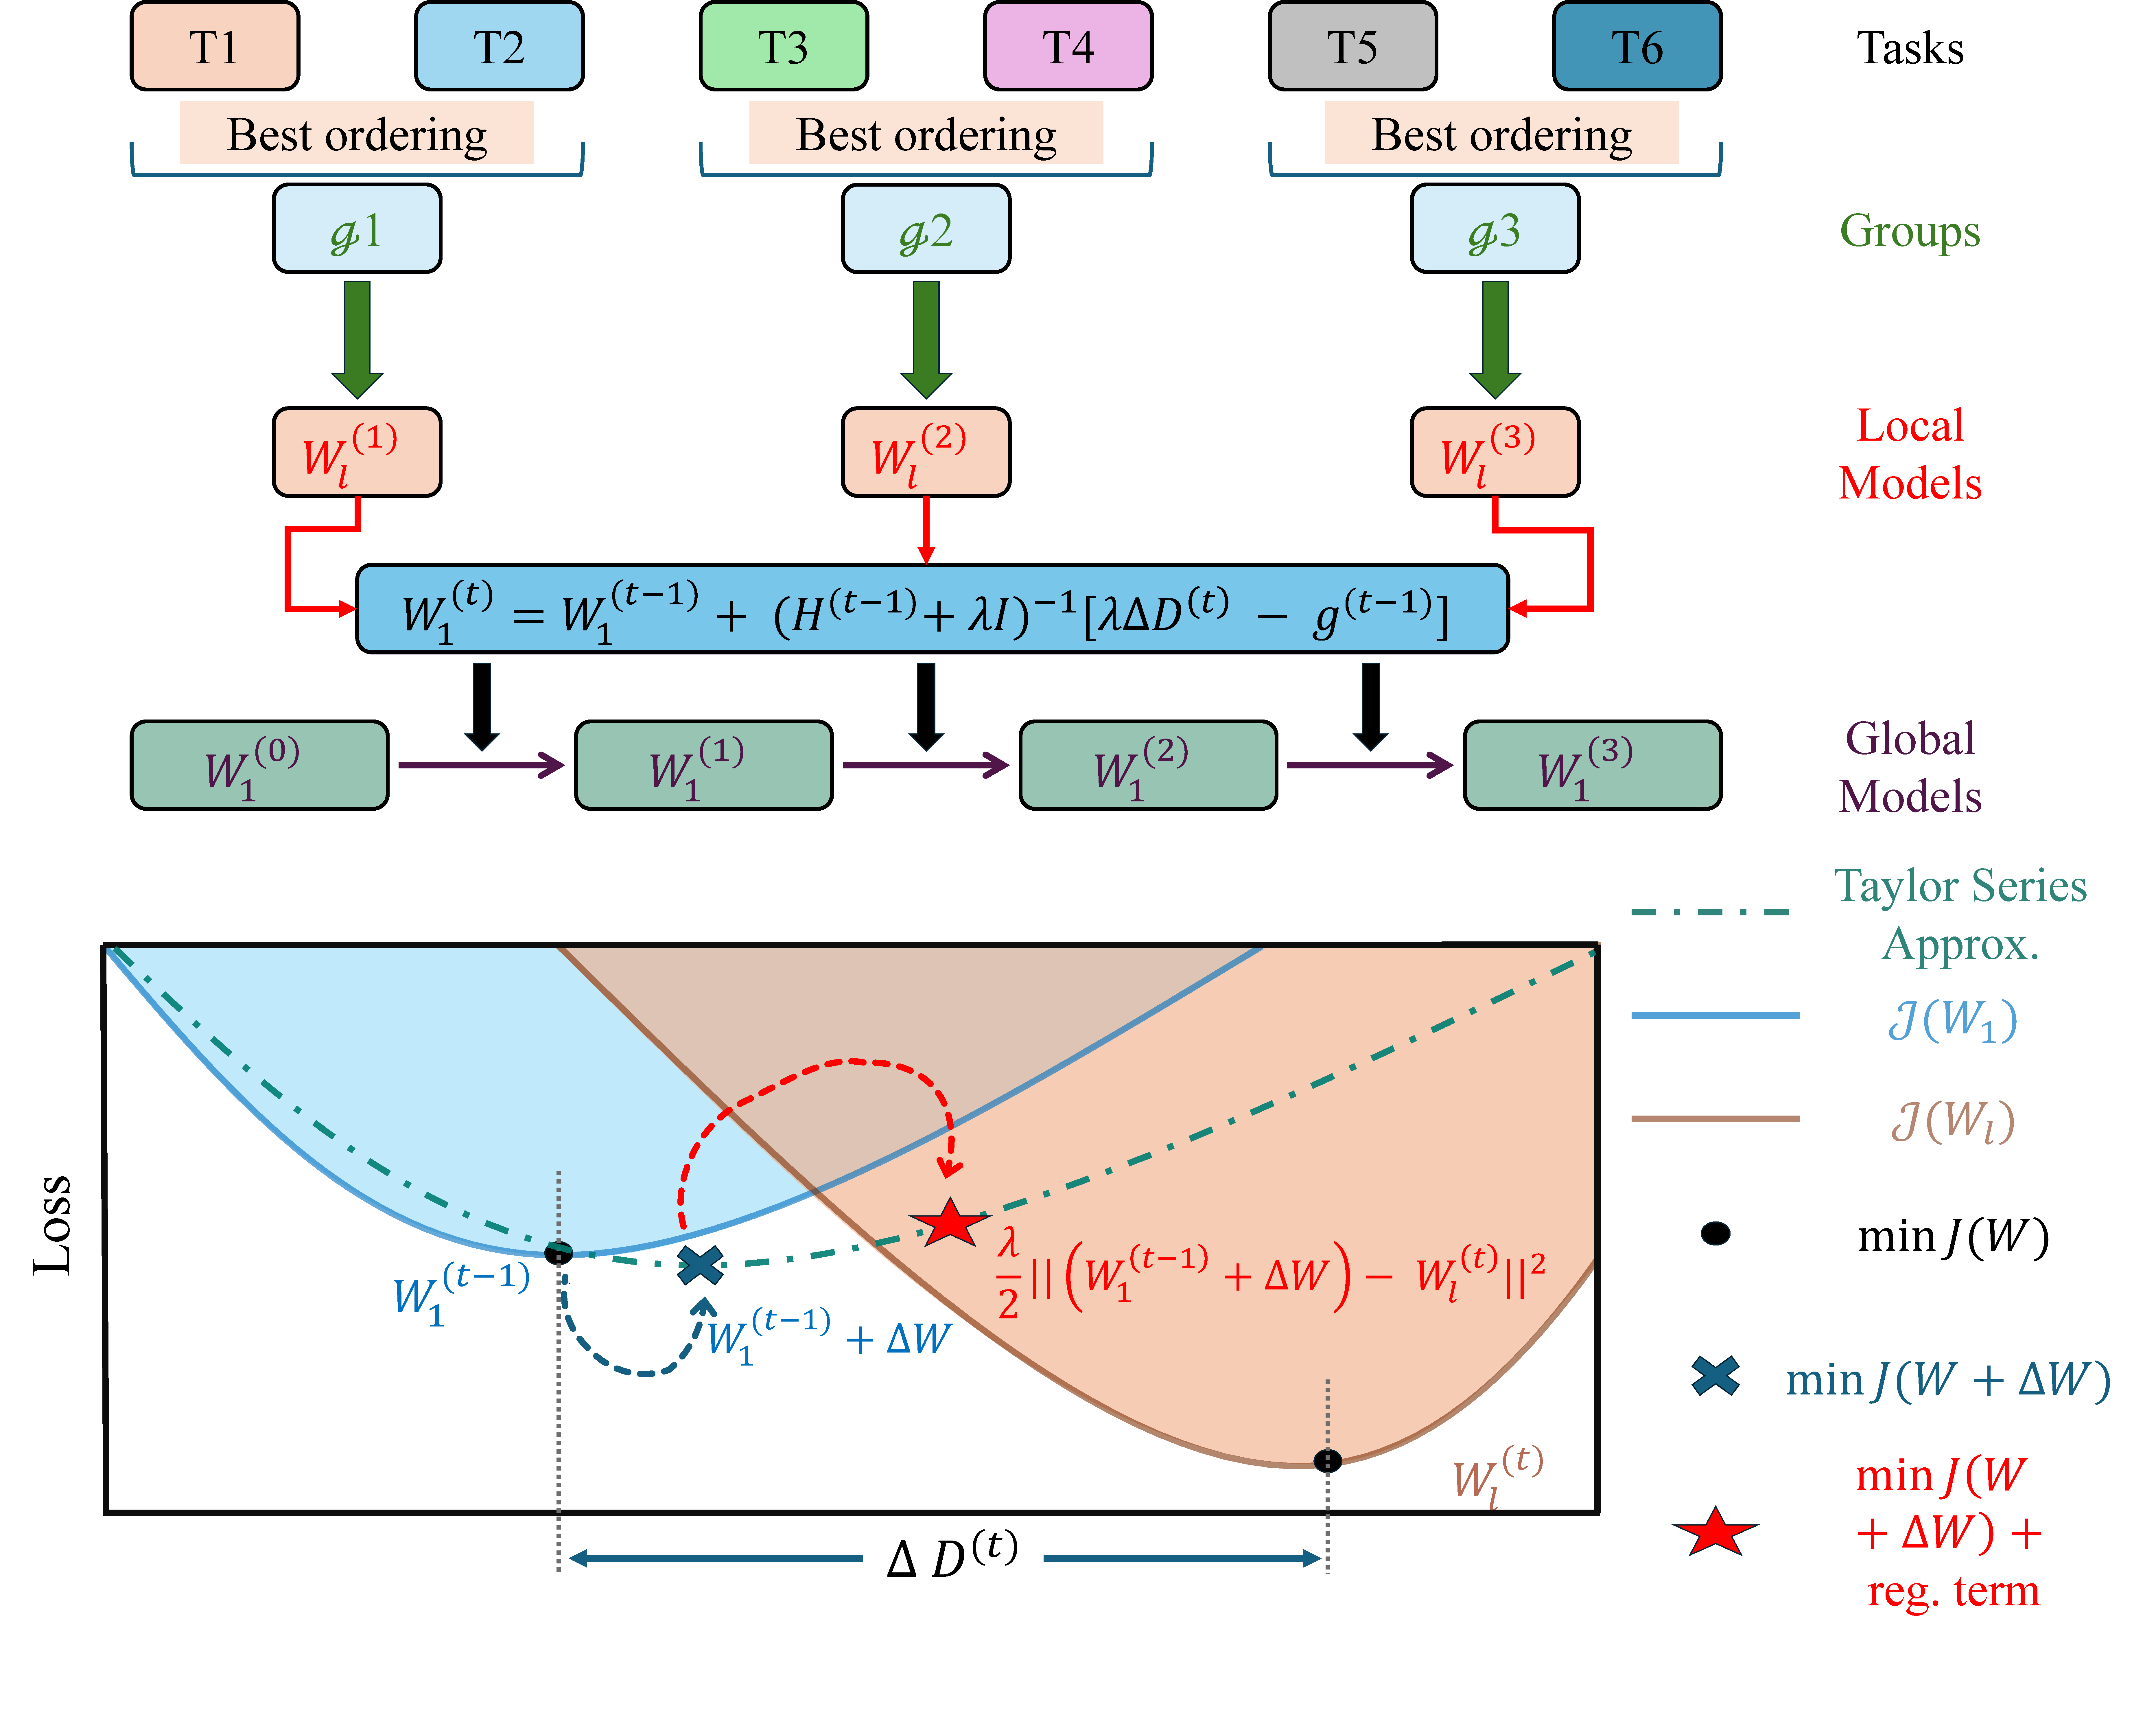
\includegraphics[width=\columnwidth]{figures/exp.pdf}
  \caption{(top)~The HTCL framework for a sequence of six tasks partitioned into three groups ($\G_1, \G_2, \G_3$). Within each group, all $\gsize!$ (here $2!$) intra-group permutations are evaluated through neural network training to provide $\wlT{1}, \wlT{2}, \wlT{3}.$ These three results are successively integrated into the hierarchical model $\whT{1}{t}$. (bottom)~Illustration of the update rule on a loss landscape. The current hierarchical model $\whT{1}{t-1}$ (blue) integrates knowledge from the local model $\wlT{t}$ (brown). Rather than naively minimizing $\J(\w)$, HTCL approximates $\J(\whT{1}{t-1}+\Dw)$ (blue cross) using a second-order Taylor expansion of the loss around $\whT{1}{t-1}$ with a regularization term that penalizes deviation from $\wlT{t}$. 
    This yields the updated hierarchical model $\whT{1}{t}$ (red star).}
    \label{fig:htcl-overview}
\end{figure}

Each hierarchical level progressively smooths and consolidates information from the faster layers below it. Lower levels (smaller $i$) retain adaptability to recent tasks, while higher levels (larger $i$) maintain long-term stability through slower updates. Empirically, we find that deeper hierarchies (e.g., $\nlev=3$) provide improved resistance to catastrophic forgetting, particularly in long task sequences. Quantitative results and ablation studies are provided in Section~\ref{sec:results}. Beyond the empirical evidence, two theoretical results underpin HTCL's design. Theorem~\ref{thm:perf-bound-main} establishes an accuracy floor relative to random task ordering, and Proposition~\ref{thm:tradeoff-main} formalizes the trade-off between permutation-search cost and marginal accuracy gain as a function of group size $k$. 

\begin{theorem}[Performance bound]
\label{thm:perf-bound-main}
HTCL's performance is never worse, in expectation, than encountering tasks in a uniformly random order. The best intra-group permutation selected within each group provides a guaranteed accuracy floor that random arrival cannot beat in expectation, and typically yields strictly better performance. Full statement and proof in Appendix~\ref{app:performance-bounds}.
\end{theorem}

\begin{proposition}[Complexity--performance trade-off] 
\label{thm:tradeoff-main}
The cost of intra-group permutation search grows linearly with the group size $\gsize$, while the marginal accuracy gain decays factorially. Most of the available improvement is therefore captured at small group sizes ($\gsize{=}2$ or $\gsize{=}3$), and larger groups buy negligible accuracy at substantial computational cost. Full derivation and assumptions in Appendix~\ref{app:proof_tradeoff}; Appendix~\ref{app:break-even-point} empirically confirms the break-even at $\gsize{=}3$ on SplitMNIST.
\end{proposition}

\begin{remark}[Time and space complexity]
\label{rem:complexity}
The exact curvature-aware update in \eqref{eq:hier_update-main} requires forming and inverting a $\pdim \times \pdim$ Hessian, resulting in worst-case time $\Theta(\pdim^3)$ and memory $\Theta(\pdim^2)$ (or $\Theta(\nlev \pdim^3)$ and $\Theta(\nlev \pdim^2)$ for an $\nlev$-level hierarchy). In practice, HTCL employs scalable second-order approximations (e.g., diagonal Hessian approximation and group size $\gsize < 5$) which reduce both time and memory to near-linear. Complete derivations and comparisons with other CL methods are provided in Appendix~\ref{app:complexity}.
\end{remark}